% -*- latex -*-
%%%%%%%%%%%%%%%%%%%%%%%%%%%%%%%%%%%%%%%%%%%%%%%%%%%%%%%%%%%%%%%%
%%%%%%%%%%%%%%%%%%%%%%%%%%%%%%%%%%%%%%%%%%%%%%%%%%%%%%%%%%%%%%%%
%%%%
%%%% This text file is part of the lecture slides for
%%%% `Parallel Computing'
%%%% by Victor Eijkhout, copyright 2012-6
%%%%
%%%% ForkJoin-slides.tex : slides about OpenMP's fork-join model
%%%%
%%%%%%%%%%%%%%%%%%%%%%%%%%%%%%%%%%%%%%%%%%%%%%%%%%%%%%%%%%%%%%%%
%%%%%%%%%%%%%%%%%%%%%%%%%%%%%%%%%%%%%%%%%%%%%%%%%%%%%%%%%%%%%%%%

\frame{\frametitle{Computer architecture terminology}
  One cluster node:

  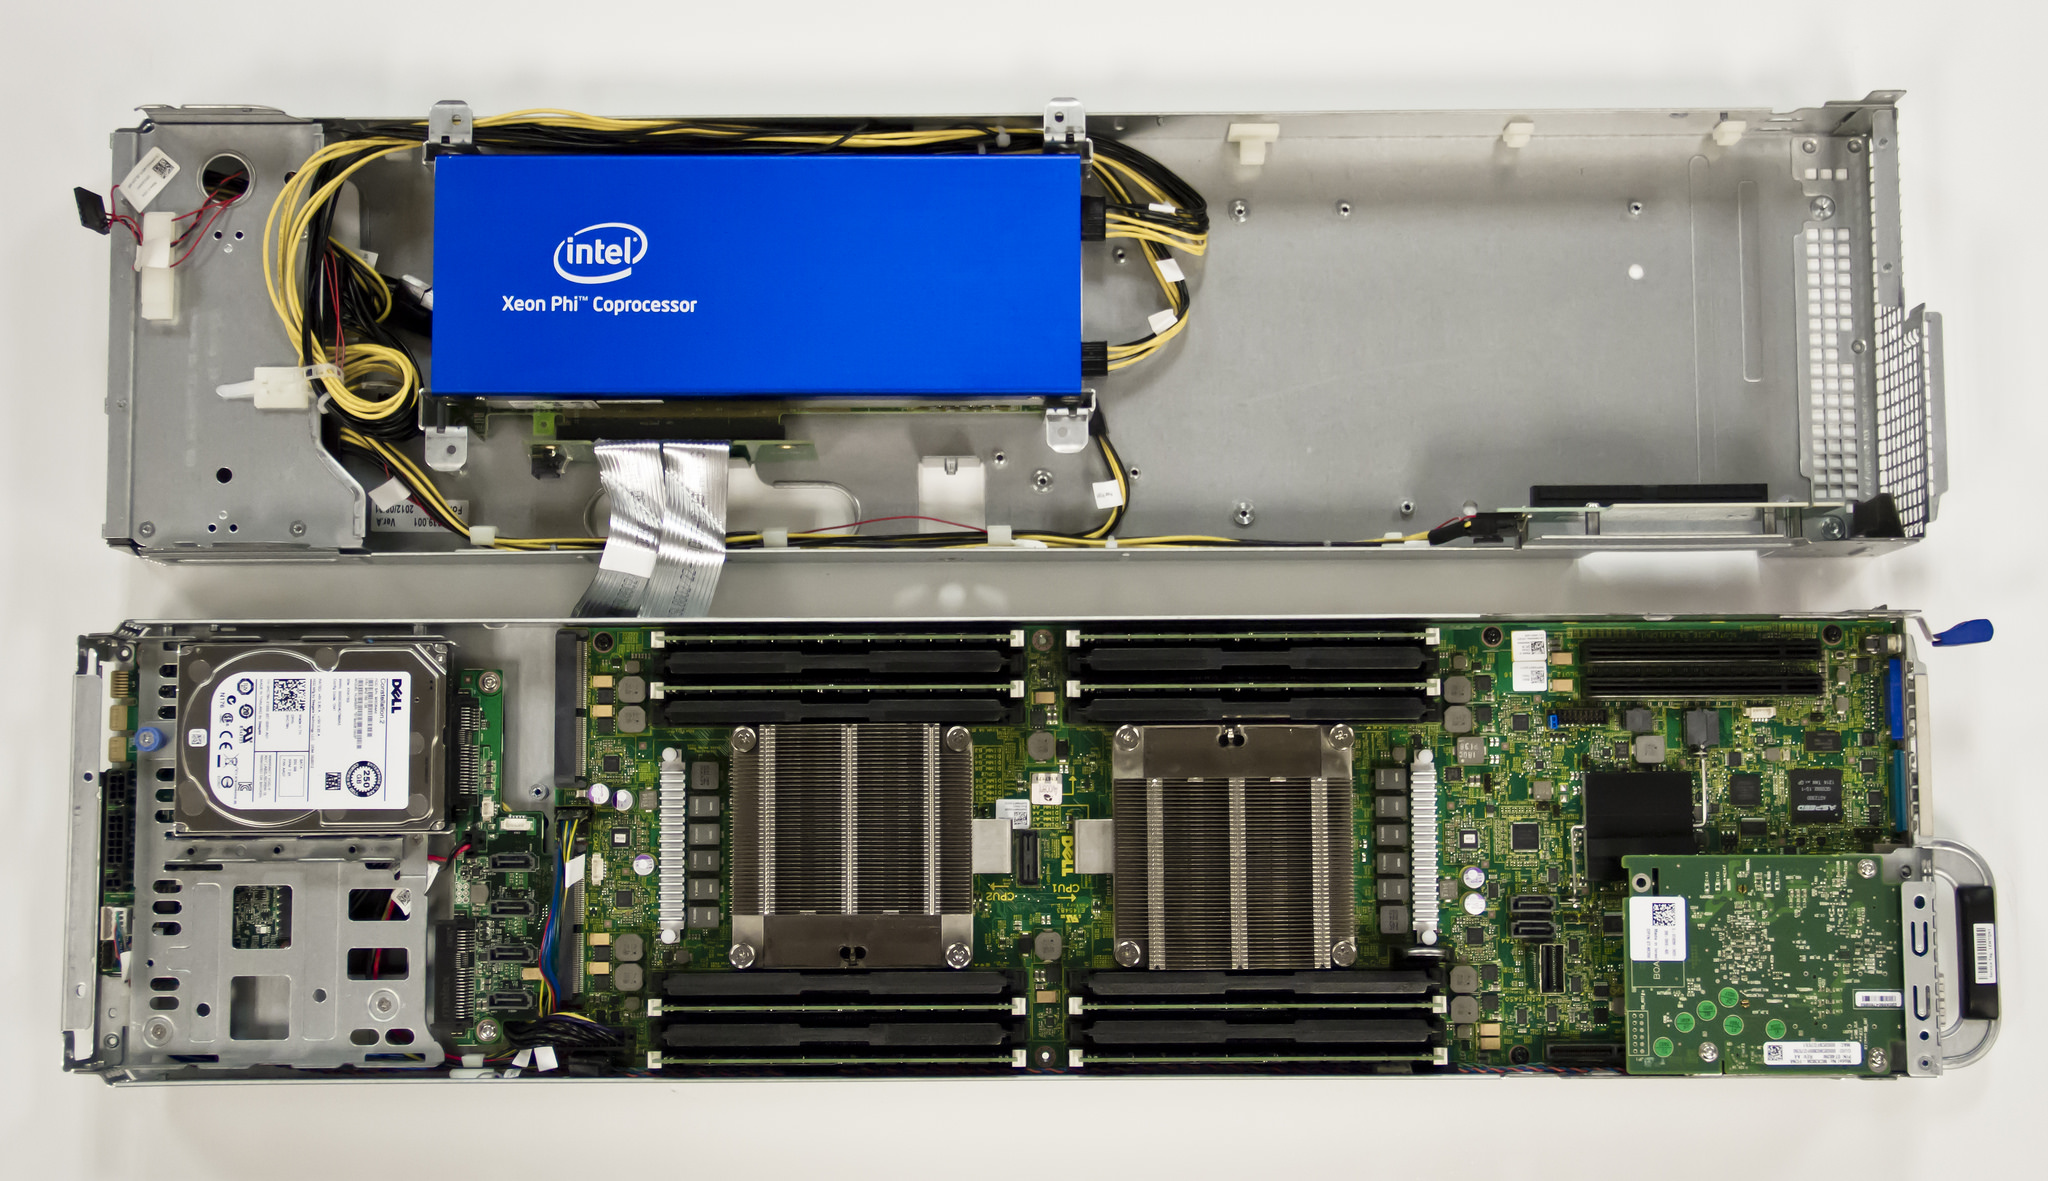
\includegraphics[scale=.13]{stampede-node}

  A node will have 1 or 2 or (sometimes) 4 `sockets': processor
  chips.\\
  There may be a co-processor attached.
}

\frame{\frametitle{Structure of a socket}

    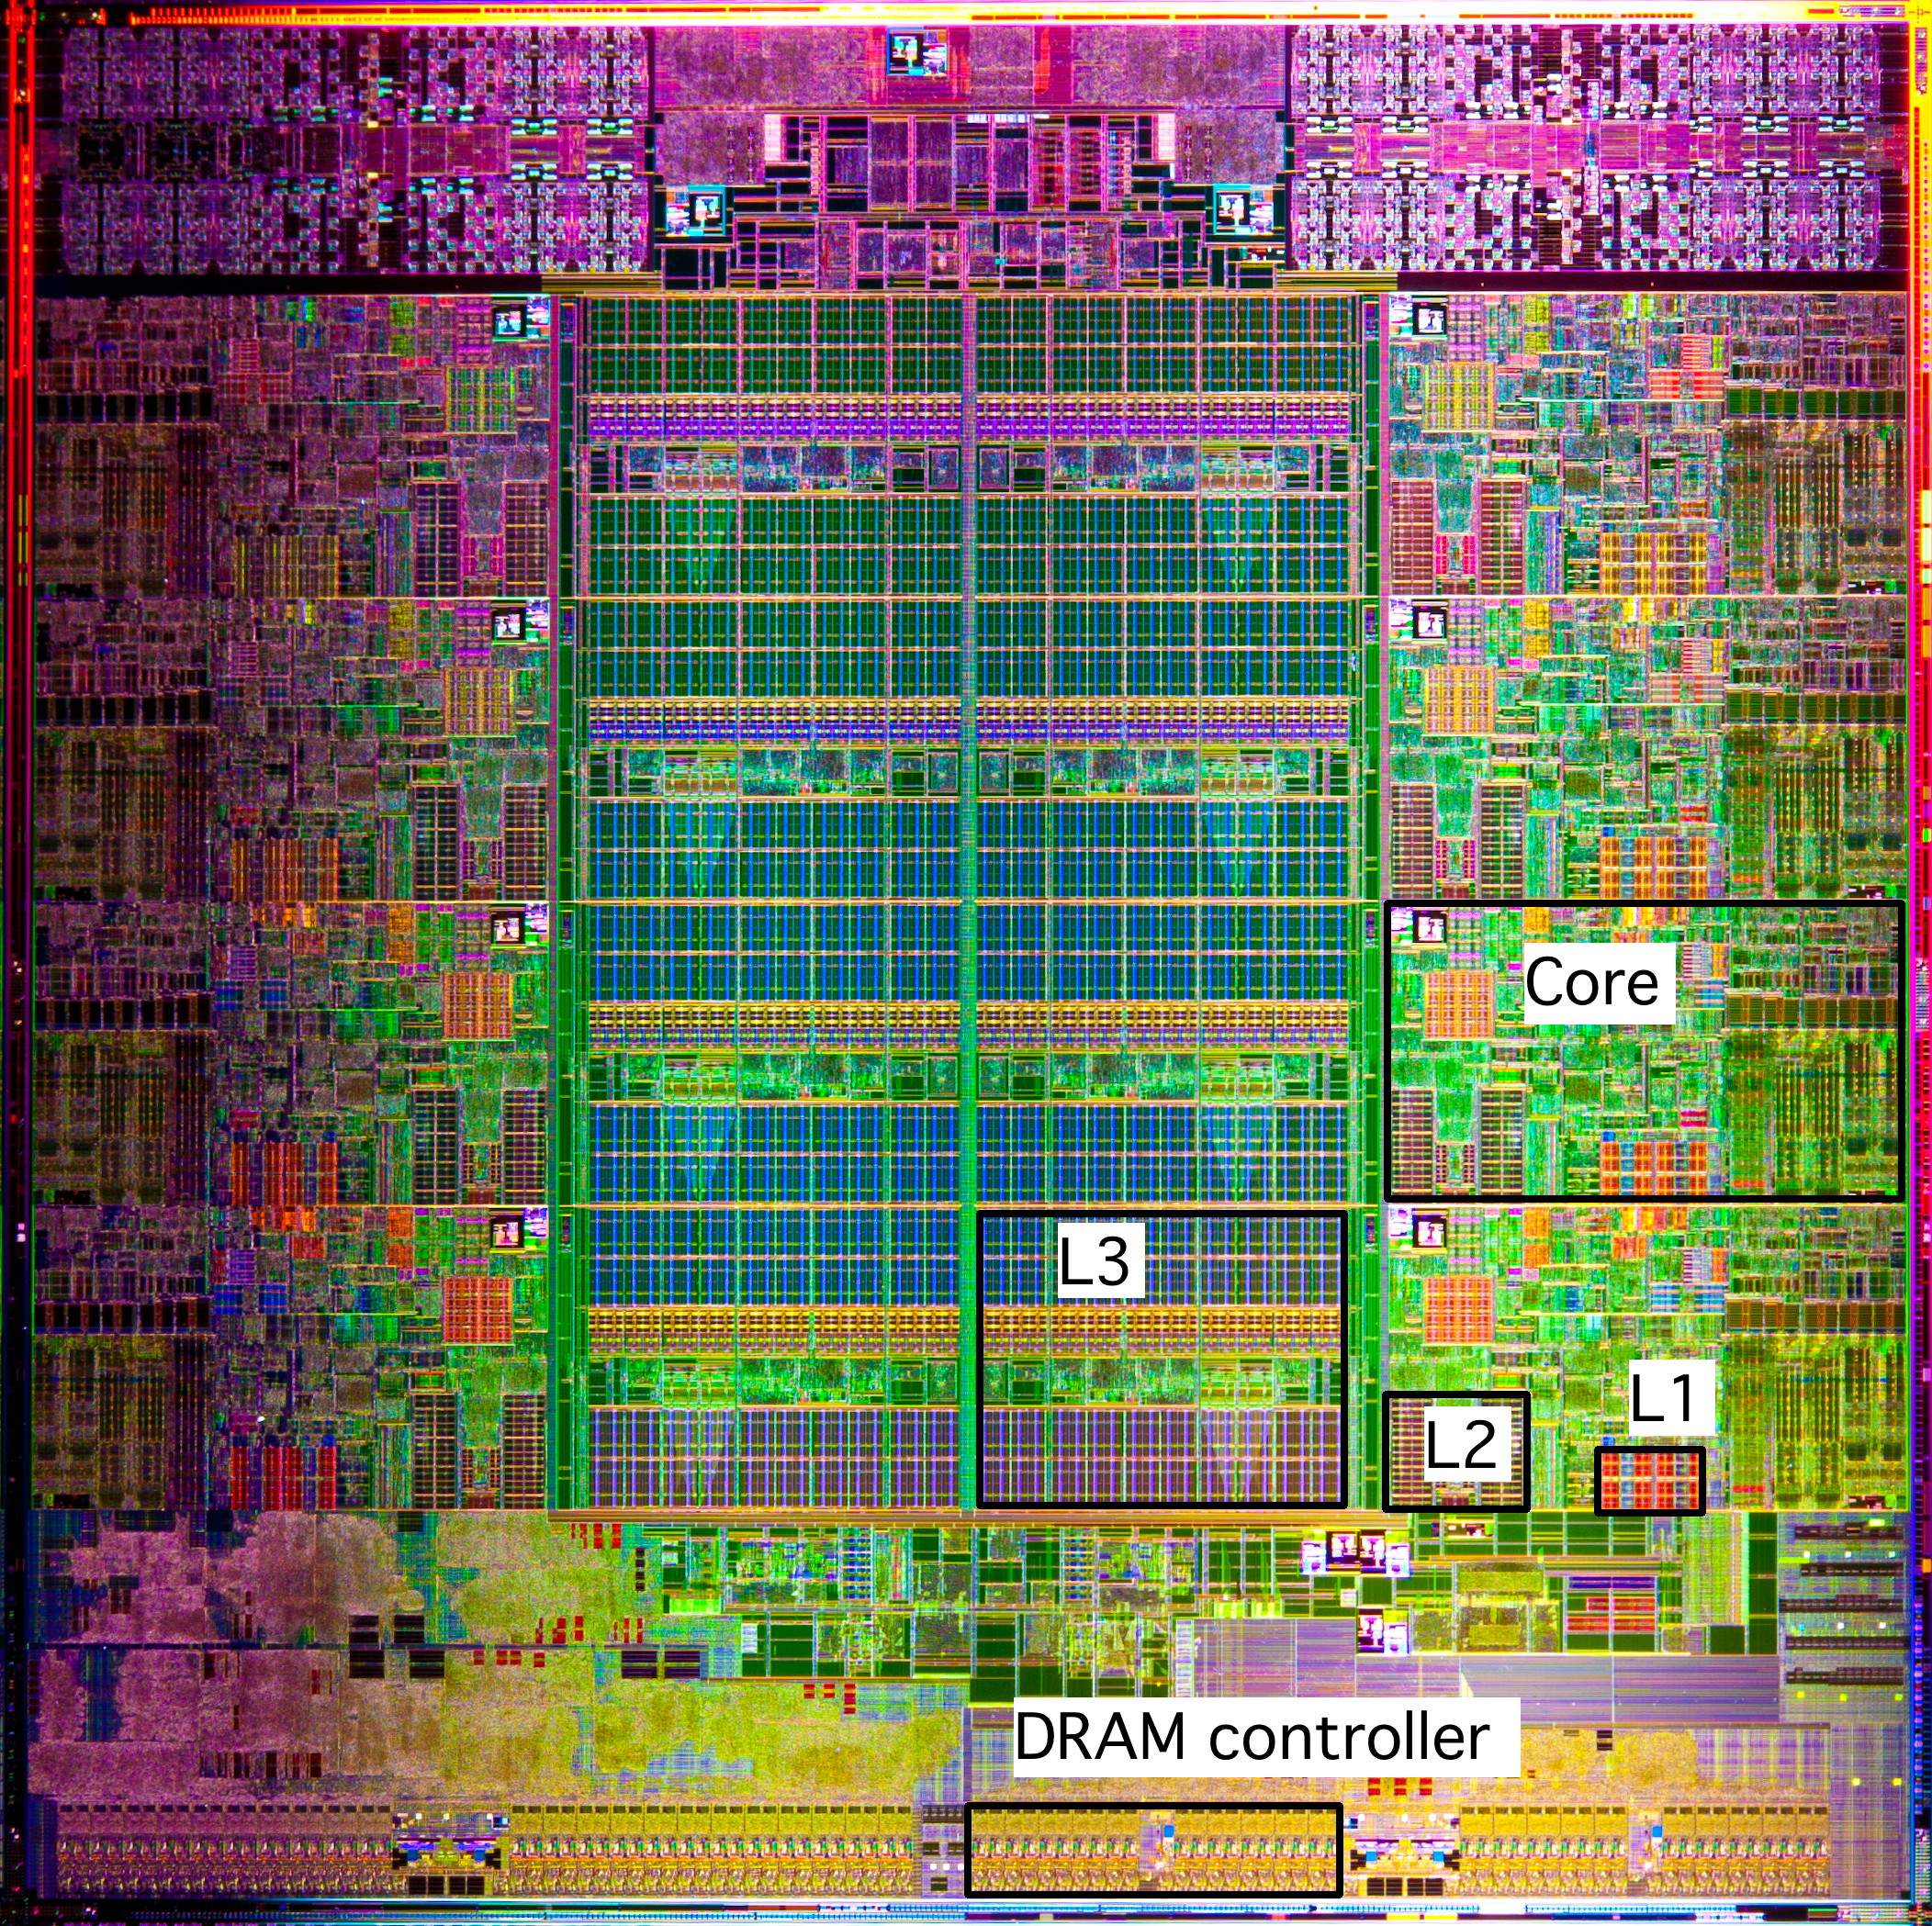
\includegraphics[scale=.25]{sandybridge-eightcore-ann}

    Eight cores per socket, making 16 per node.\\
    They all access the same data.
}

\begin{frame}{Threads}
  Process: stream of instructions\\
  Thread: process can duplicate itself, same code, access to same data

  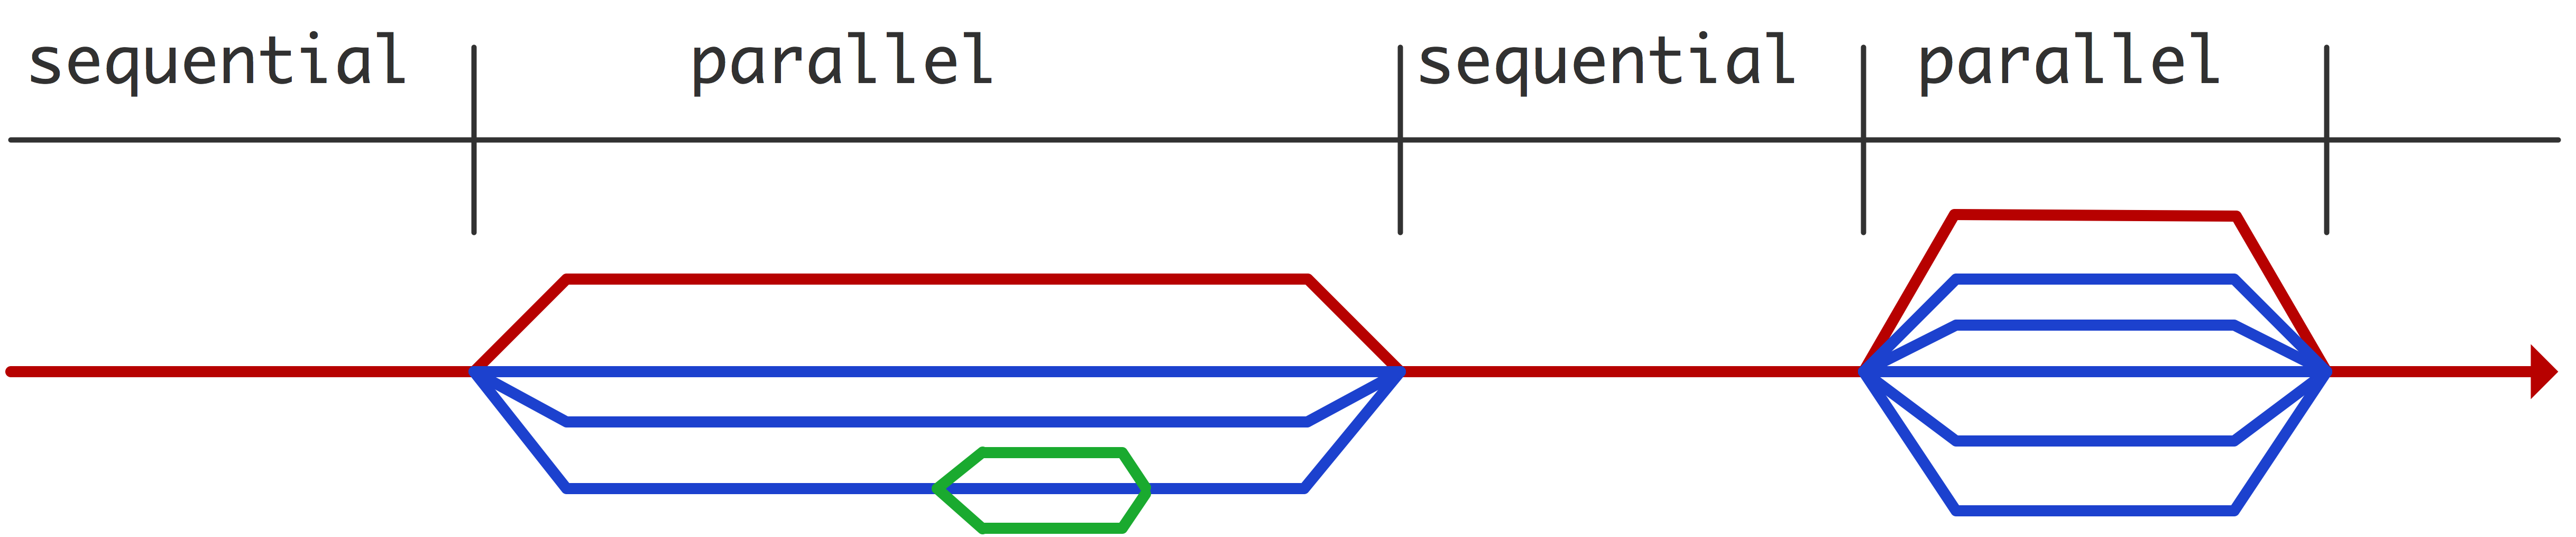
\includegraphics[scale=.07]{fork-join}

  The OS will place threads on different cores: parallel
  performance.\\
  Note: threads are software. More threads than cores or fewer is allowed.
\end{frame}

\begin{frame}[containsverbatim]{To write an OpenMP program}
\begin{verbatim}
#include "omp.h"
\end{verbatim}
in C, and 
\begin{verbatim}
use omp_lib
\end{verbatim}
or
\begin{verbatim}
#include "omp_lib.h"
\end{verbatim}
for Fortran.  
\end{frame}

\begin{frame}[containsverbatim]{To compile an OpenMP program}
\begin{verbatim}
# gcc
gcc -o foo foo.c -fopenmp
# Intel compiler
icc -o foo foo.c -openmp
\end{verbatim}
\end{frame}

\begin{frame}[containsverbatim]{To run an OpenMP program}
\begin{verbatim}
export OMP_NUM_THREADS=8
./my_omp_program
\end{verbatim}

\begin{tacc}
  Stampede has 16 cores; more than 16 threads does not make sense.
\end{tacc}

Quick experiment:
\begin{verbatim}
for t in 1 2 4 8 12 16; do
  OMP_NUM_THREADS=$t ./my_omp_program
done
\end{verbatim}
\end{frame}

\begin{exerciseframe}[parallel]
  \input ex:omp-procthread
\end{exerciseframe}

\begin{frame}{What happens if I press that button?}
  Who of you has tried setting the number of threads (much) larger
  than the number of cores? What happened?
\end{frame}

\begin{frame}[containsverbatim]{Threads and threads}
  \begin{itemize}    
  \item Threads are software, cores are hardware.
  \item The OS can move threads between cores: not a good idea for
    performance.
  \item Set: \n{export OMP_PROC_BIND=true} and you'll be good in
    most of the cases.
  \item Look up `affinity' in the OMP standard for all the details.
  \end{itemize}
\end{frame}

\begin{exerciseframe}
  \input ex:omp-procthreadn
\end{exerciseframe}

\begin{frame}[containsverbatim]{Shared memory problems}
Race condition: simultaneous update of shared data:
\begin{tabbing}
  process 1: \texttt{I=I+2}\\
  process 2: \texttt{I=I+3}
\end{tabbing}
Results can be indeterminate:

\tiny
\begin{tabular}{|rr|rr|rr|}
  \hline
  \multicolumn{2}{|c|}{scenario 1.}& \multicolumn{2}{|c|}{scenario 2.}&
  \multicolumn{2}{|c|}{scenario 3.}\\ \hline
  \multicolumn{6}{|c|}{$\n{I}=0$}\\ \hline
  read $\n{I}=0$&read $\n{I}=0$&
    read $\n{I}=0$&read $\n{I}=0$&
      read $\n{I}=0$& \\
  compute $\n{I}=2$&compute $\n{I}=3$& 
    compute $\n{I}=2$&compute $\n{I}=3$&
      compute $\n{I}=2$& \\
  write $\n{I}=2$& & &write $\n{I}=3$&write $\n{I}=2$& \\
  &write $\n{I}=3$&write $\n{I}=2$& & &read $\n{I}=2$\\
  &&&&&compute $\n{I}=5$\\
  &&&&&write $\n{I}=5$\\
  \hline
  \multicolumn{2}{|c|}{$\n{I}=3$}& \multicolumn{2}{|c|}{$\n{I}=2$}&
  \multicolumn{2}{|c|}{$\n{I}=5$}\\ \hline
\end{tabular}
\end{frame}

